\begin{frame}{Digital Images}
    \begin{itemize}
    \itemsep = 1em
        \item<1-> Image are 2D arrays of dimensions $M\times N$
        \item<1-> Each \emph{pixel} $(i,j)$ takes values in $\{0,1,\ldots,255\}$
        \item<2-> \colorbox{LightGreen}{Image histogram} gives the number of pixels that take a particular intensity\\
        \visible<3->{$h[k]$ is the count of the pixels that take the intensity level $k$}
        \item<4-> Normalised histogram $p[k] = \displaystyle\frac{1}{MN}h[k]$
    \end{itemize}
\end{frame}

\begin{frame}{Which has `Better' Contrast?}
    \only<1>{
    \begin{figure}
        \subfigure[Image 1]{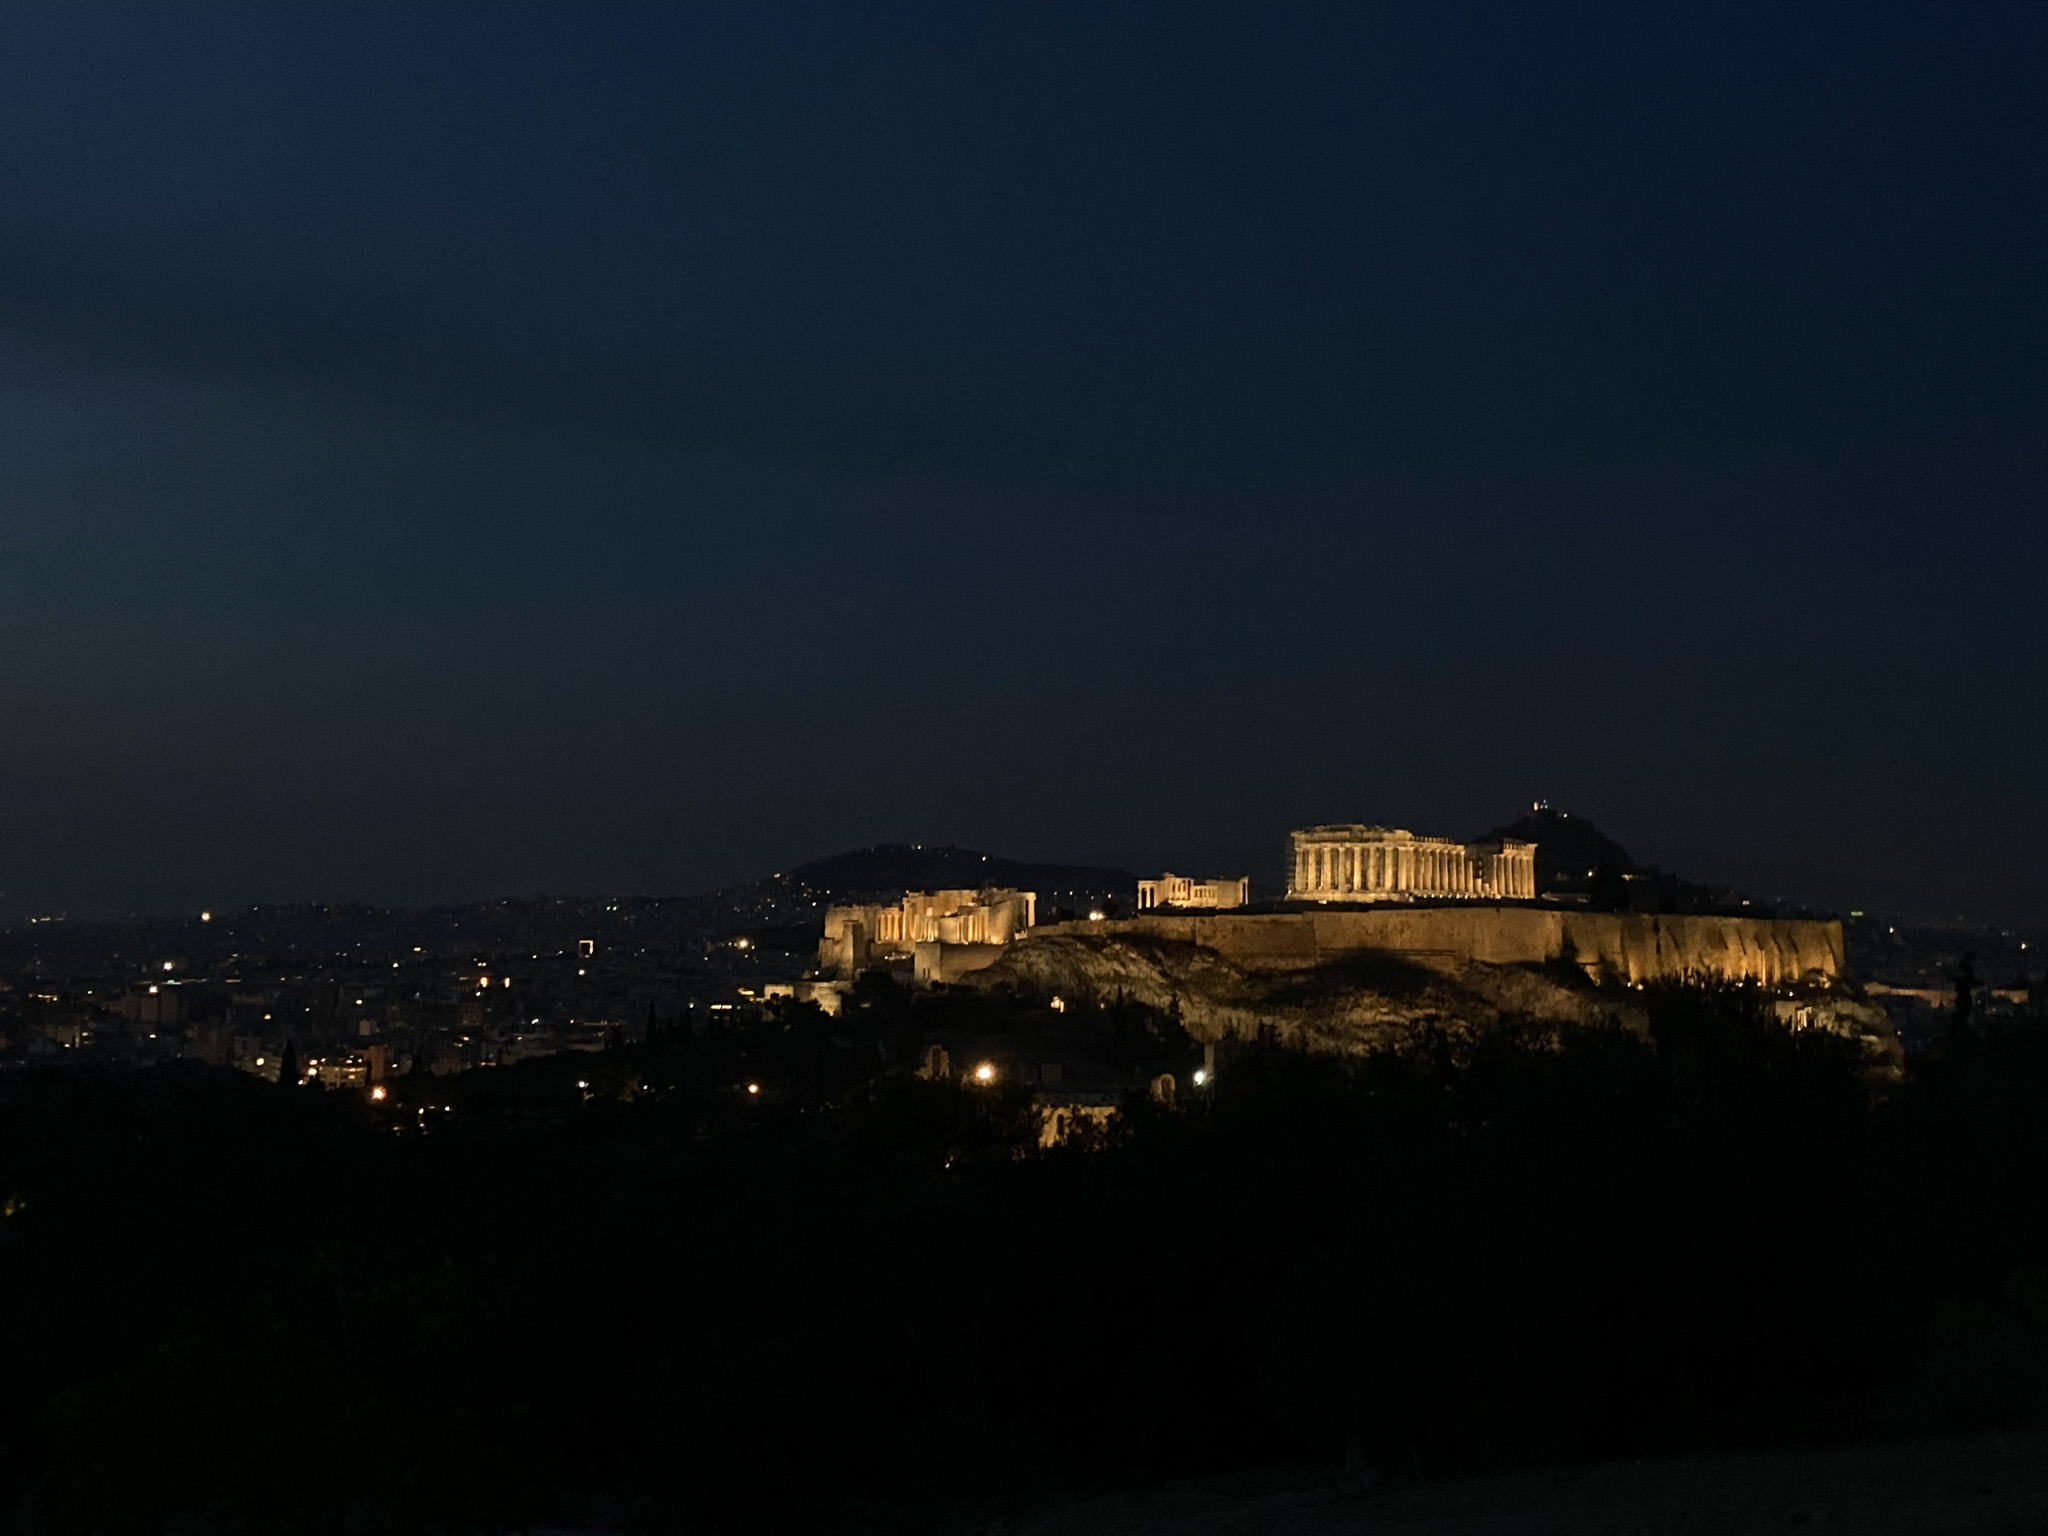
\includegraphics[width=2.5in]{../data/image-1.jpg}}
        \subfigure[Image 2]{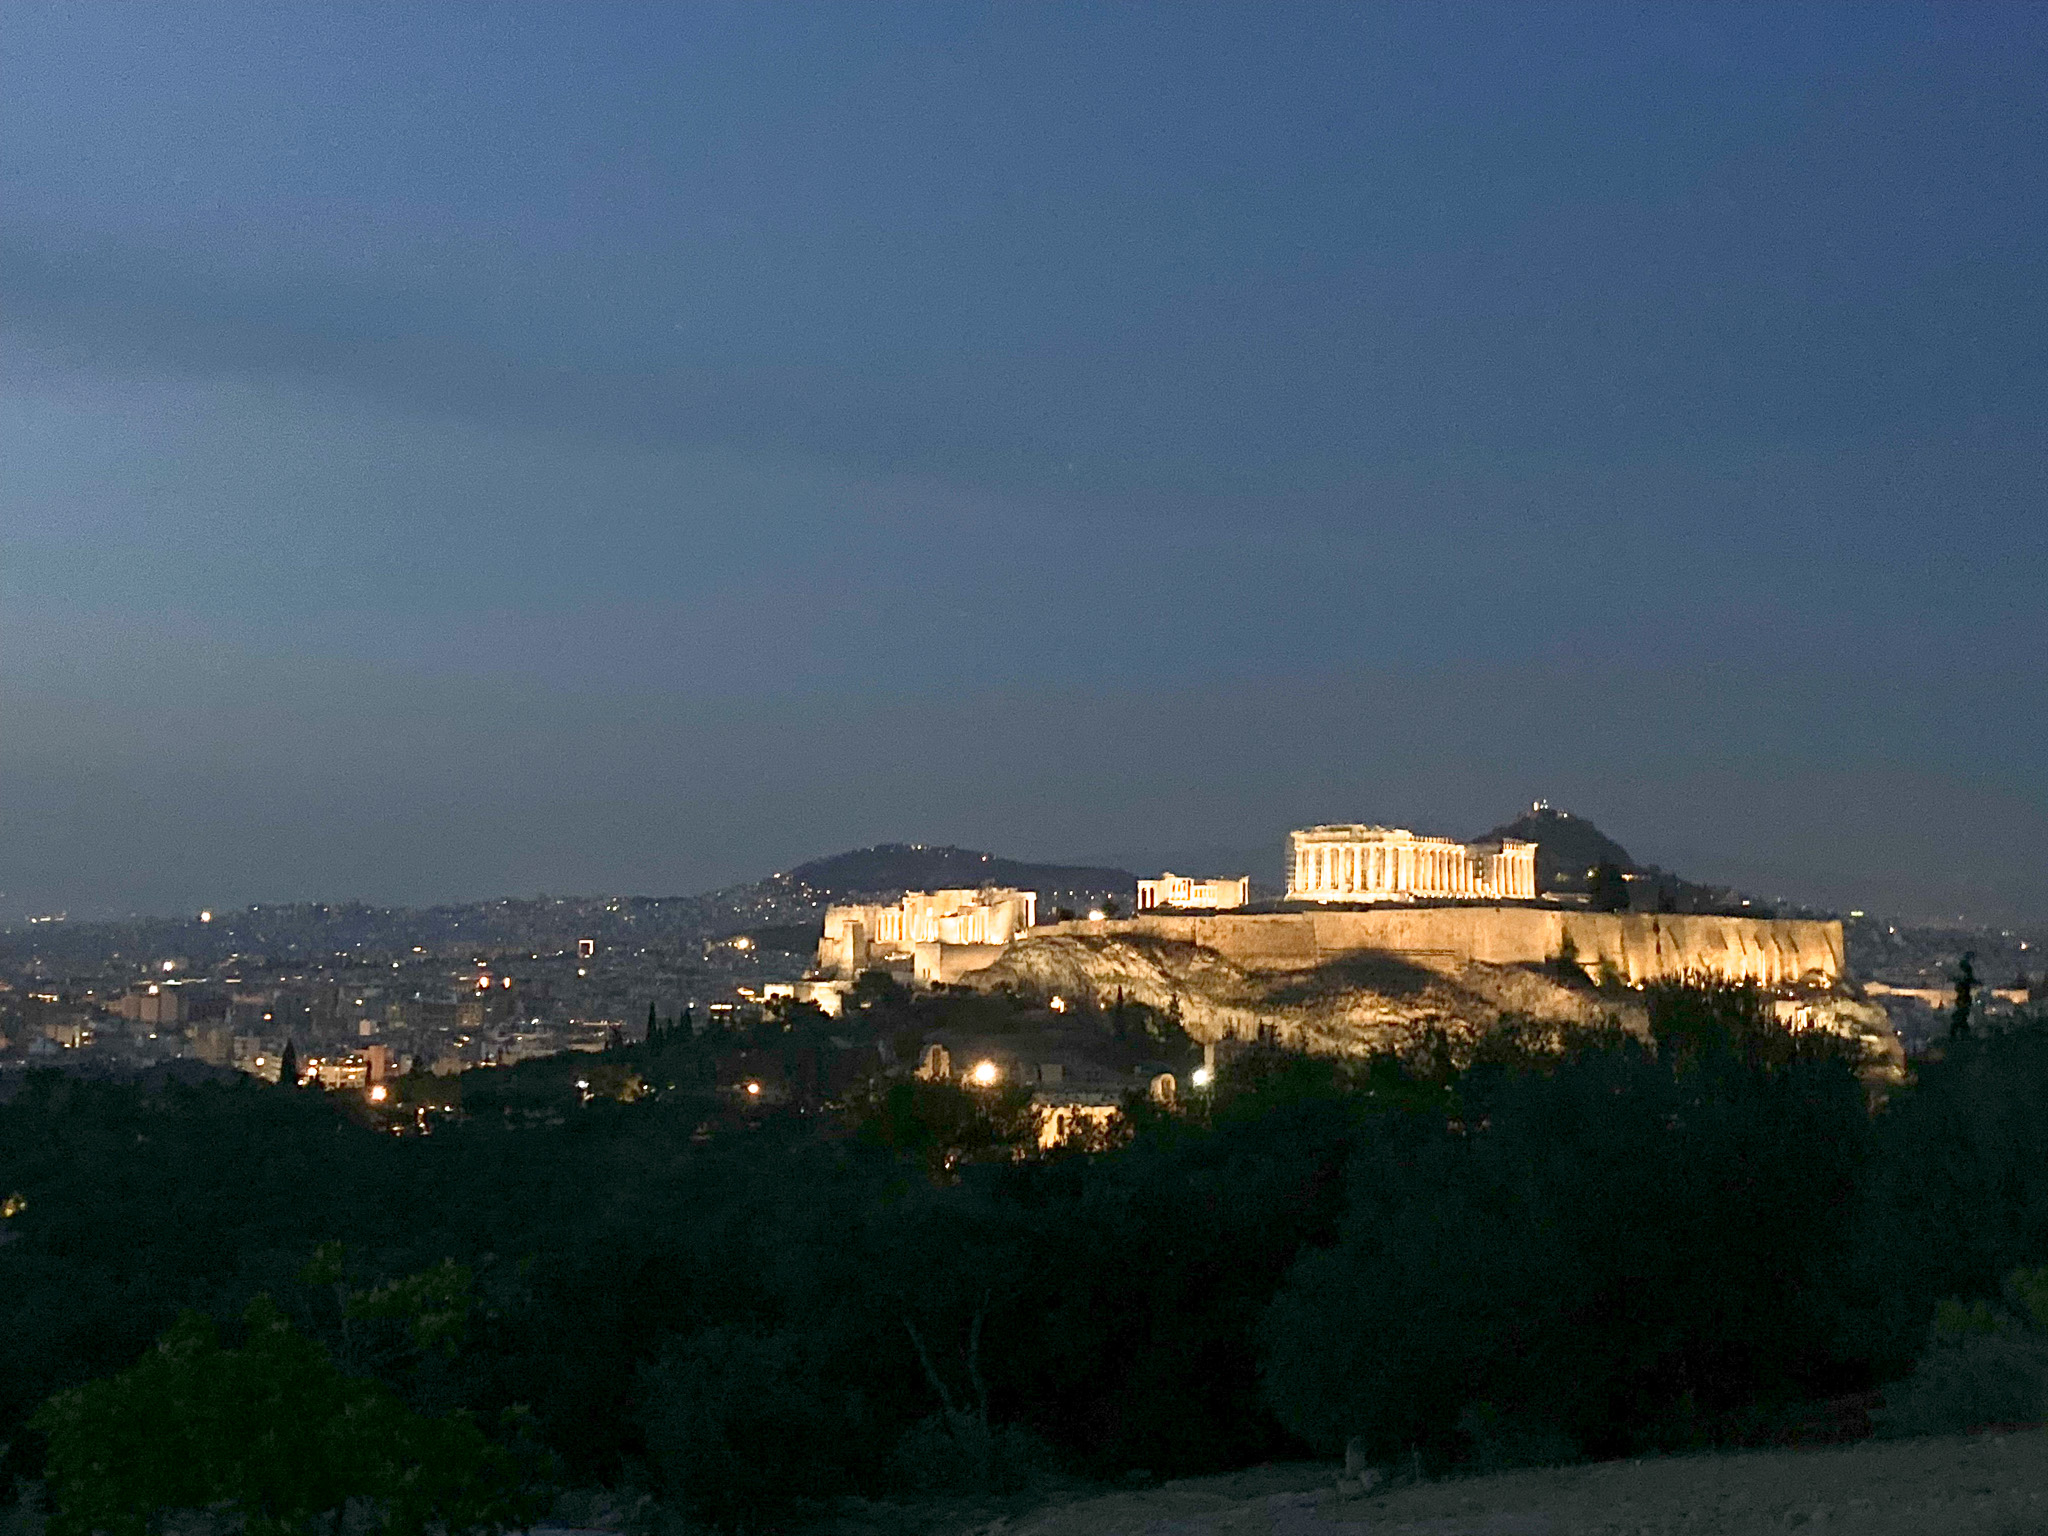
\includegraphics[width=2.5in]{../data/image-2.jpg}}
        % \caption{Flat histogram gives better contrast.}
    \end{figure}
    }
    \only<2>{
    \begin{figure}
        \subfigure[Histogram of Image 1]{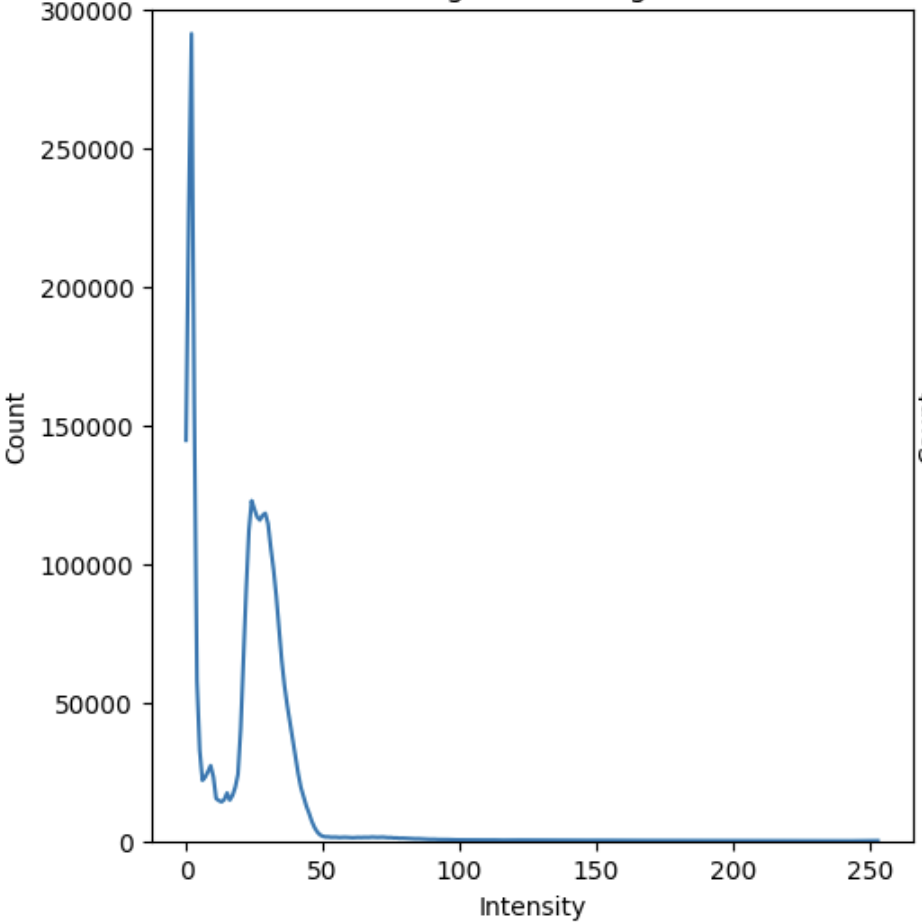
\includegraphics[width=2.3in]{../data/hist-image-1.png}}
        \subfigure[Histogram of Image 2]{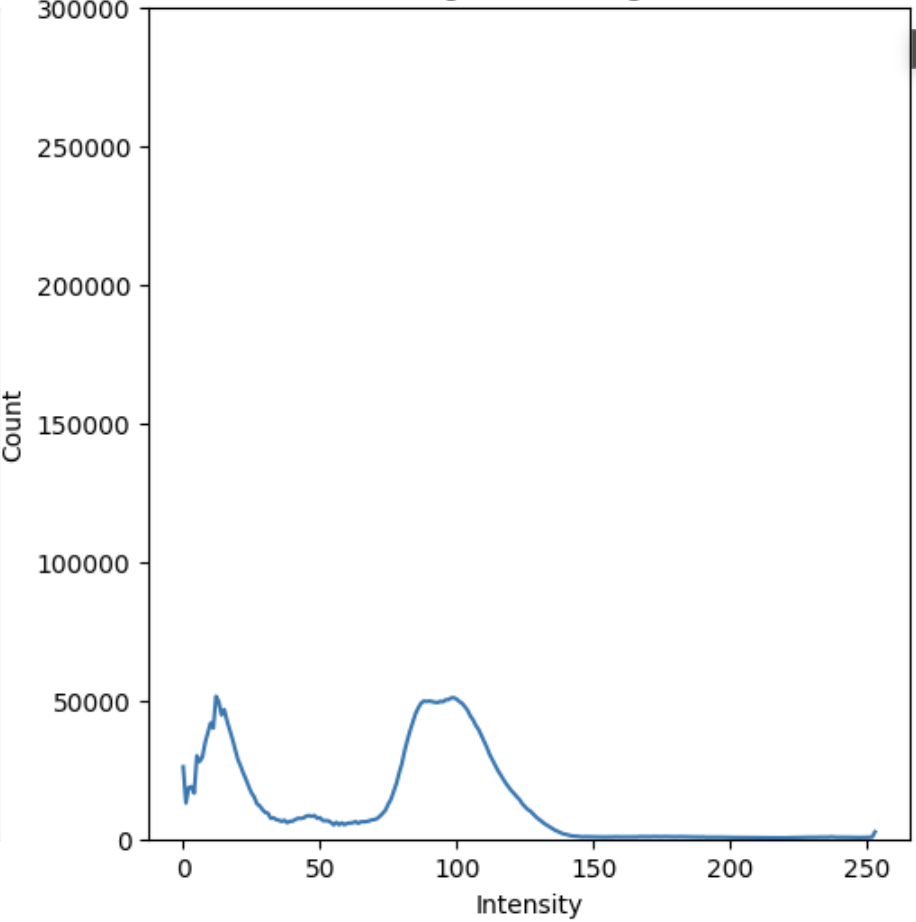
\includegraphics[width=2.3in]{../data/hist-image-2.png}}
        \caption{Flat histogram $\implies$ better contrast.}
    \end{figure}
    }
\end{frame}

\begin{frame}{Histogram Equalisation}
    \visible<1->{
    \begin{lemma}
        Let $X$ be a continuous random variable with an invertible cumulative distribution function $F_X$, and let $Y = F_X(X)$. Then, $Y = \cl U[0,1]$.
    \end{lemma}
    }
    \visible<2->{
        \begin{proof}
        Since $Y = F_X(X)$, $0\leq Y\leq 1$.
            \begin{align*}
                \forall y\in [0,1], \; F_Y(y) &= P[Y\leq y], \\
                &= P[F_X(X)\leq y],\\
                &= P[X\leq F_X^{-1}(y)],\\
                &= F_X(F_X^{-1}(y)) = y.
            \end{align*}
        Therefore, $Y = \cl U[0,1]$.
        \end{proof}
    }
\end{frame}

\begin{frame}{Discrete Implementation of Histogram Equalisation}
    \begin{itemize}
    \itemsep=1em
        \item<1-> Given image $I[i,j]$
        \item<1-> Compute the normalized histogram $p[k]$\\
        Note: $p[k]$ is the relative number of pixels with intensity $k$
        \item<2-> Histogram equalisation
        \coloredeq{J[i,j] = \displaystyle\sum_{k=0}^{I[i,j]} p[k]}
        \item<3-> \alert{Warning: Not all distribution functions are invertible; discrete implementations introduce errors; output histogram may not be the uniform distribution.}
    \end{itemize}
\end{frame}

\begin{frame}{}
  \centering
  \LARGE\emph{Fin.}
  \vspace*{1em}

  
\includegraphics[width=2.75in]{./figures/calvin-hobbes-01.jpeg}
\end{frame}